\section{Magnetostatic Analysis}

\textbf{Magnetic vector potential \\ \\}
In case when the electric field does not depend on time the following can be written
\begin{equation*}
	\nabla \cdot \vec{B} = 0
\end{equation*}
\begin{equation*}
	\nabla \times \vec{H} = \vec{J}
\end{equation*}
Due to the fact that a divergence of a curl is always equal to zero, it is possible in this case to represent the magnetic flux density as a curl of a vector function 
\begin{equation*}
	\vec{B} = \nabla \times \vec{A}
\end{equation*}
which is called the magnetic vector potential. It must fulfil the following partial differential equation
\begin{equation*}
	\underbrace{\underbrace{\nabla \times \left(\frac{1}{\mu}\underbrace{\nabla \times \vec{A}}_{\bot}\right)}_{\bot} = \vec{J}}_{||}
\end{equation*}
If the material is homogeneous, the last equation could be further simplified as 
\begin{equation*}
	\Delta\vec{A} = -\mu \vec{J}
\end{equation*}

\textbf{\\ Boundary Value Problem (BVP)\\}
\begin{minipage}[lt]{11cm}
	\begin{tabular}{l}
		\textbf{3D:} \\
		\(\displaystyle \nabla \times \left(\frac{1}{\mu}\nabla \times \vec{A}\right) = \vec{J} \) \\
		\(\displaystyle \vec{n} \times \vec{A} = 0, \textrm{ over } \partial_D\Omega \) \\
		\(\displaystyle \vec{n} \times \nabla \times \vec{A} = 0,\textrm{ over } \partial_N\Omega \) \\
		\textbf{2D planar (from book):} \\
		\(\displaystyle -\frac{\partial }{\partial x} \left(\frac{1}{\mu} \frac{\partial A_z}{\partial x}\right) - \frac{\partial }{\partial y} \left(\frac{1}{\mu} \frac{\partial A_z}{\partial y}\right) = J_z \) \\
		\(\displaystyle A_z = 0, \textrm{ over } \partial_D\Omega \) \\
		\(\displaystyle \frac{\partial A_z}{\partial n} = 0, \textrm{ over } \partial_N\Omega\) \\
		\textbf{First, the current density $\vec{J}$ must be computed to obtain a magnetostatic solution.}
	\end{tabular}
\end{minipage}
\begin{minipage}[rt]{8cm}
	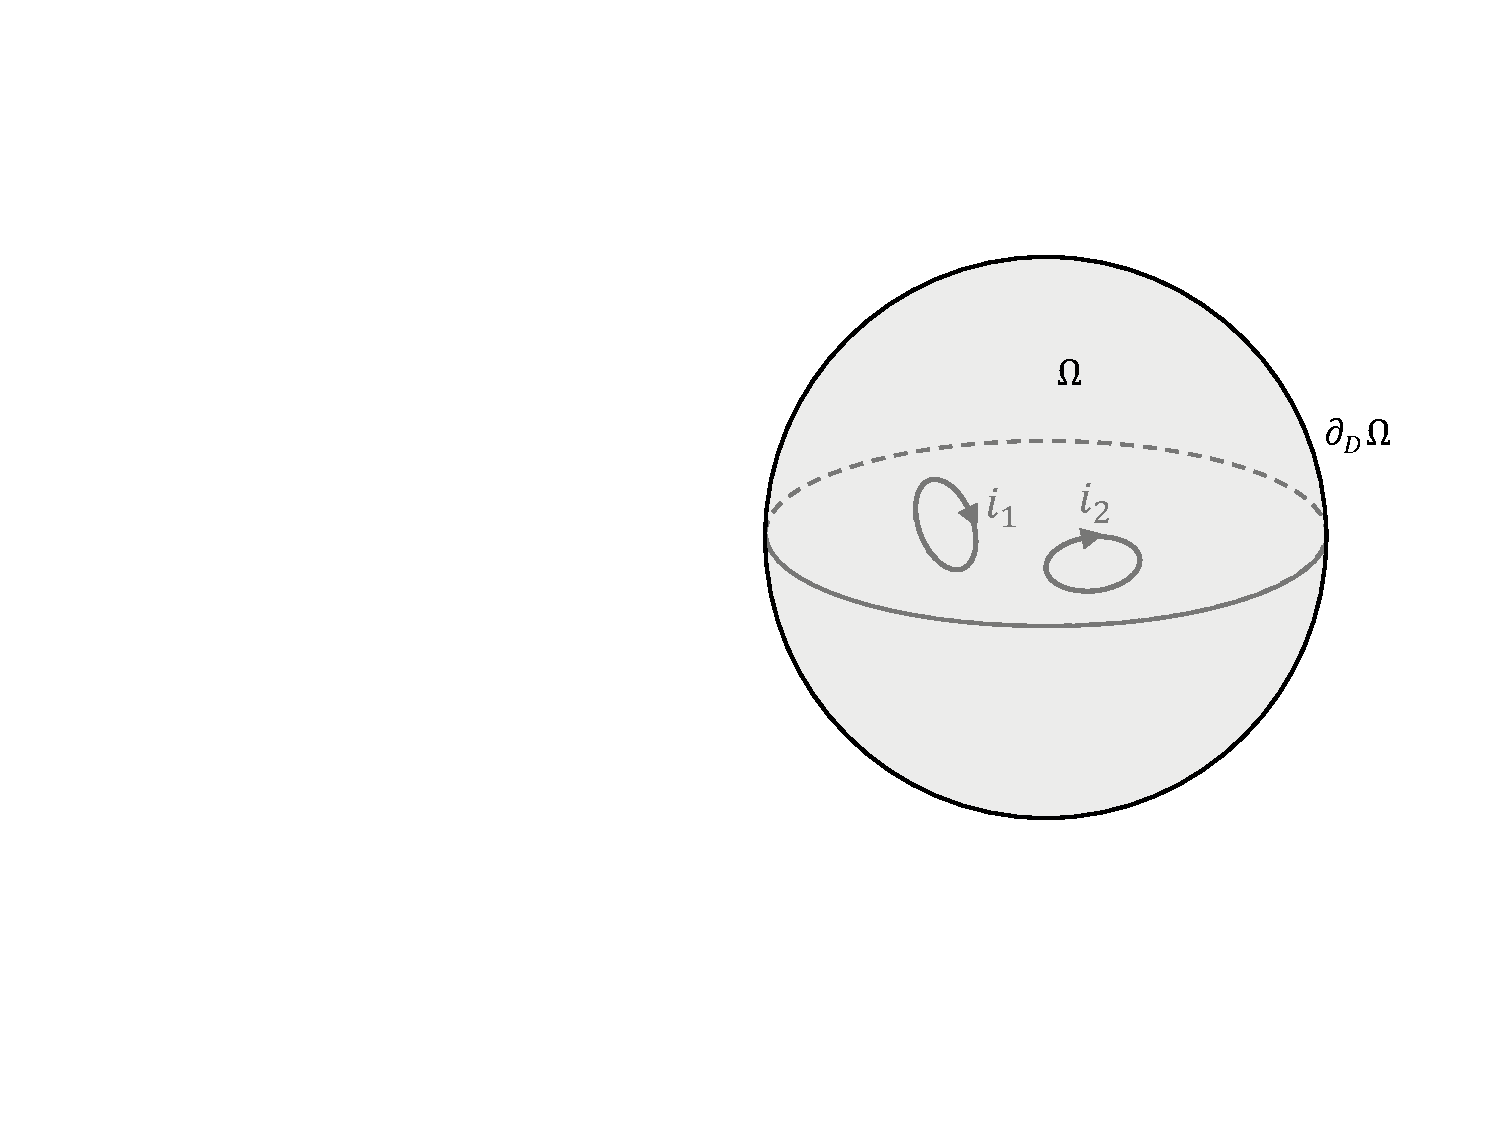
\includegraphics[width=.8\textwidth]{./images/BVP_magnetostatic.pdf}
\end{minipage}

\textbf{\\ \\ Post processing \\ }
\begin{tabular}{ll}
	Magnetic energy $\left[Ws\right]$: & \(\displaystyle W_m = \frac{1}{2} \iiint\limits_{\left(\Omega\right)} \vec{B} \cdot \vec{H} dV \) \\
	Inductivity $\left[H\right]$: & \(\displaystyle L = \frac{2 W_m}{I^2} \) 
\end{tabular}